\documentclass{article}

\usepackage{mathtools}

\numberwithin{equation}{subsection}

\usepackage{amsthm}

\theoremstyle{remark}
\newtheorem*{remark}{Remark}

\usepackage{gensymb}
\usepackage{minted}
\usepackage{graphicx}
\usepackage{float}

\usepackage{titling}

\predate{}
\postdate{}


\newcommand{\qtotal}{q_{\mathrm{total}}}

\newcommand{\DeltaT}{\Delta{}T}
\newcommand{\DeltaTmax}{\DeltaT_{\mathrm{max}}}
\newcommand{\Deltarfh}{\Delta{}r_{fh}}

\newenvironment{definitiontable}{
\renewcommand{\arraystretch}{1.5}
\begin{tabular}{lp{0.8\textwidth}}
}
{
\end{tabular}
\renewcommand{\arraystretch}{1.0}
}

\title{How Big Do I Make My Heat Exchangers?}
\date{}

\begin{document}

\maketitle

\section{Basic Heat Exchanger Design}

We consider heat exchangers of the following basic form.

\begin{figure}[H]
\centering
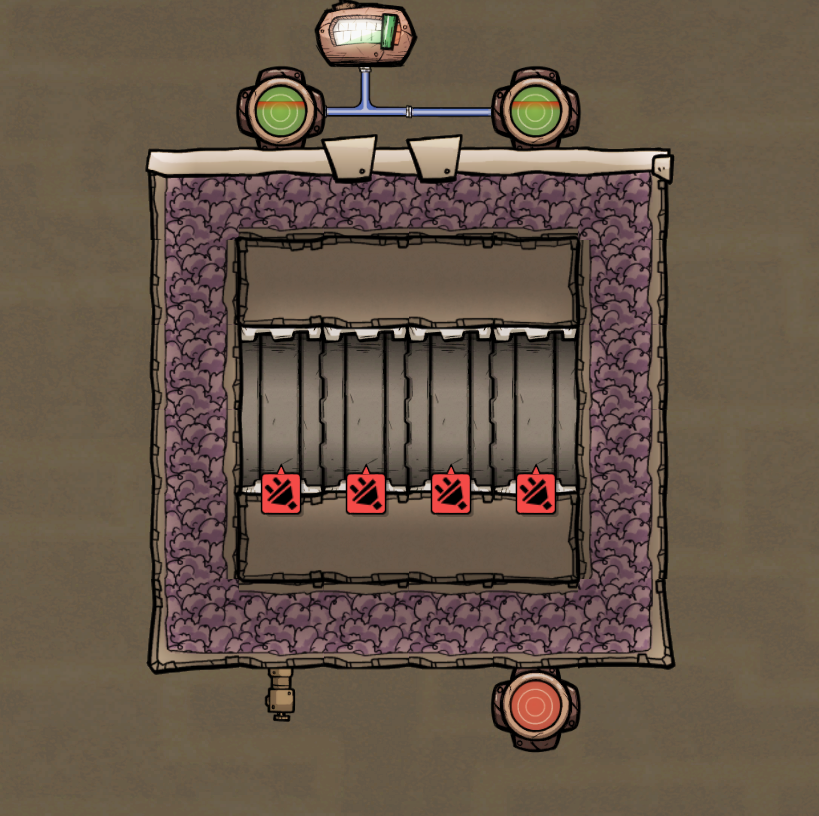
\includegraphics[width=0.5\textwidth]{Basic Passive Heat Exchanger Main Overlay}
\caption{A 4-tile long heat exchanger designed to uses piped coolant on both sides.}
\end{figure}

The tiles are meant to act as a thermal buffer, and the mechanized airlocks allow for precision control over the heat passing through the radiator.
We allow for more than one layer of tiles beyond the heat exchanger, and we allow for asymmetry in the number of tiles and choices of materials.

Although pipes are shown in the image, conveyor rails are also supported, as well as stationary mass simply adjacent to the outer tiles of the exchanger (often this would be a liquid or a gas).
Waterfalls and flowing gas is also supported, provided that appropriate an appropriate flow rate can be provided.

When designing heat exchangers, we often know what materials we will use and how we want the exchanger to interact with the materials to be heated or cooled.
We also typically know what temperatures we can tolerate on either side of the exchanger.
What we don't usually know is how large the heat exchanger needs to be in order to move enough heat from one side of the other without violating those temperature constraints, given the interfaces and materials used.
The script assists in finding this quantity.

\section{Script Model}

The script makes a distinction between a hot side and a cold side.
Heat is assumed to move from the hot side to the cold side.
Each side can have different paramters and a different interface.

The different interfaces available are \emph{stationary}, \emph{waterfall}, and \emph{conduits}.

\begin{itemize}
\item The \emph{stationary} interface is used when heat exchanger is butted up against some stationary mass of a constant temperature, which may be solid, liquid, or gas.

\item The \emph{waterfall} interface is used when the heat exchanger is being used to cool cells of flowing fluid (liquid or gas).
The flowing cells are directly adjacent to the outermost tiles on the heat exchanger.
The ratio of heat exchanger tiles contacting coolant cells over heat exchanger tiles not contacting coolant cells can be specified to accomodate the use of bead flows.

\item The \emph{conduits} interface is used when the coolant is being piped through a conduit of some sort (a liquid/gas pipe, or a conveyor rail).
\end{itemize}

When speficying the temperature constraints of flowing coolants, either the entry or exit temperatures may be specified.
The script will also auto-detect which tiles/pipes you mean to build by inspecting the materials used as coolant and the materials used to construct them.

\section{Example Usage}

\subsection{Cool Steam Vent}

We have a cool steam vent that outputs 110 \degree{}C steam that we want to cool just enough that it condenses.  We use liquid pipes carrying polluted water as coolant at ~95 \degree{}C to cool the steam as it comes out of the vent.

The worst-case steam vent outputs \(3 \frac{\mathrm{kg}}{\mathrm{s}}\) water 50 out of 60 seconds during the active period, which is 20 out of every 25 cycles.  If we cool the steam down to 95 \degree{}C as fast as it can come out of the vent while actively emitting, that's \(188055 \frac{\mathrm{DTU}}{\mathrm{s}}\).

We'll assume that the other side of the heat exchanger is hooked up to an aquatuner on a loop that also cools some other machines.
If this aquatuner is set to cool the polluted water down to -19 \degree{}C, then the worst-case temperature on the output side of this heat exchanger should be 9 \degree{}C.
This worst-case assumes that the cool steam vent is the last thing on the coolant loop, the aquatiner powering the loop is fully loaded when all machines are accounted for, and the coolant packets have a nasty habit of just barely not heating up enough to pass through the aquatuner safely.

We'll assume early game materials for the heat exchanger, so copper ore for the mechanized airlocks, copper for the pipes, and granite for the tiles.

\begin{minted}[breaklines]{bash}
./heatexchanger.py calculate -H 188.055 --hot-coolant-entry-temperature 95 --cold-coolant-exit-temperature 9
1.0660942609551771
\end{minted}

As it happens, most people's heat exchangers for taming cool steam vents are probably seriously overbuilt.

\subsection{Early-Game Metal Refinery}

We want to refine steel at full duty-cycle, but we're using a cold biome as our heat sink.

Steel produces 93566480 DTU per recipe, or \(2339162 \frac{\mathrm{DTU}}{\mathrm{s}}\) when running at full throttle.
If we're using polluted water as the coolant, it'll heat up 55.974Kelvin.
The hottest temperature we can support with polluted water is 119.25 \degree{}C.
Let's set the coolant temperature going into the metal refinery at 60 \degree{}C, making the output temperature 115.974 \degree{}C.

On the other side, we just have some cold mass made out of tiles.
Let's assume that we've wise built this thing under some ice/polluted ice at something like -40 \degree{}C.

We'll start with early game materials for the heat exchanger, so copper ore for the mechanized airlockis, copper for the pipes, granite for the tiles.

\begin{minted}[breaklines]{bash}
./heatexchanger.py calculate -H 2339.162 --hot-interface conduits --hot-coolant-exit-temperature 60 --cold-interface stationary --cold-coolant 'Polluted Ice' --cold-coolant-temperature -40
13.534572745642086
\end{minted}

Ice will quickly melt when subjected to the heat output of refining steel, and water has a lower thermal conductivity than ice.
Additionally, once we get some refined metal, we may want to upgrade the tiles connecting the water/ice to the heat exchanger so as to increase the maximum temperature that we can tolerate on the cold side before steel production becomes rate-limited.
It turns out that we can maintain our throughput at a similarly-sized heat exchanger all the way up to 55 \degree{}C in the surrounding environment.

\begin{minted}[breaklines]{bash}
$ ./heatexchanger.py calculate -H 2339.162 --hot-interface conduits --hot-coolant-exit-temperature 60 --cold-interface stationary --cold-coolant 'Polluted Water' --cold-coolant-temperature 55 --cold-tile-material Copper
13.264723299503103
\end{minted}

\section{Formulas}

The formulas used in the heat exchanger script are derived from approximate models of the heat transfer behavior in the game.
The formulas for the heat flow across the length of the radiator are conservative estimates, meaning that they'll under-estimate the heat flow given the parameters, or alternately over-estimate the reqwuired length.
The formulas for the thermal conductivity are merely approximate.
As such, some caution is advised when building heat exchangers that are very close to the estimated required length.

\subsection{Definitions}

\begin{definitiontable}
\(\qtotal\) & the total \(\frac{\mathrm{DTU}}{\mathrm{s}}\) that we want to transfer from the hot side to the cool side \\

\(\DeltaTmax\) & the maximum difference in temperature that we can tolerate between one side of the heat exchanger the other, in Kelvin \\

\(l\) & the length of the heat exchanger, in tiles \\

\(m_{h}\), \(m_{c}\) & the coolat mass per tile length of heat exchanger on the hot and cold sides, respectively, in \(\frac{\mathrm{g}}{\mathrm{tile}}\) \\

\(h_{h}\), \(h_{c}\) & the specific heat capacity of the coolant on the hot and cold sides, respectively, in \(\frac{\mathrm{DTU}}{\mathrm{g} \cdot \mathrm{K}}\) \\

\(f_{h}\), \(f_{c}\) & the rate of flow of the coolant on the hot and cold sides, respectively, in \(\frac{\mathrm{g}}{\mathrm{s}}\) \\

\(k\) & the thermal conductivity of a single slice (one tile of length) of the heat exchanger, in \(\frac{\mathrm{DTU}}{\mathrm{K} \cdot \mathrm{tile} \cdot \mathrm{s}}\) \\
\end{definitiontable}

\subsection{Calculating \(k\)}

Each heat exchanger has two halves, one on each side of the layer of mechanized airlocks.
Each half has a thermal conductivity determined by the configuration of the tiles/pipes w.r.t. the coolant.
The subsections below describe how to calculate the thermal resistance of half heat exchangers depending on their configuration.

The thermal conductivity of a single slice of a heat exchanger is most easily computed by modelling it as a heat circuit.
We're interested in the thermal resistance between the coolant one one side, and the coolant on the other.

Each half of the heat exchanger can have an interface chosen independently of the other, so we consider the heat exchanger as being made up of two halves, separated by the mechanized airlocks.
Each half has an equivalent resistance, which we add to the other half to get the total resistance across the heat exchanger per tile.
Thermal conductivity is the reciprocial of thermal resistance, so if \(r_{h}\) and \(r_{c}\) are the thermal resistances of the hot and cold halves, respectively, then

\begin{equation}
k = \frac{1}{r_{h} + r_{c}}
\end{equation}

\subsubsection{Cells}

When interfacing directly with cells, the only thing in-between the mechanized airlocks and the coolant/cells are tiles.
We have to account for the thermal resistance between the mechanized airlocks and the tiles, the tiles and the coolant cells, and the tiles and themselves (depending on how many layers of tiles there are).

We are given

\begin{definitiontable}
\(k_{a}\) & the thermal conductivity of the mechanized airlock material as given by the game \\

\(k_{t}\) & the thermal conductivity of the tile material as given by the game \\

\(k_{c}\) & the thermal conductivity of the cell material as given by the game \\

\(M\) & \(25\) if the cells are a gas, or \(1\) otherwise \\

\(n\) & the number of tiles past the mechanized airlocks in this half of the heat exchanger \\

\(R\) & the ratio of slices in contact with coolant cells over slices no in contact with coolant cells
\end{definitiontable}

From this we compute

\begin{definitiontable}
\(r_{a,t}\) & thermal resistance between a mechanized airlock and a tile \\

\(r_{t,c}\) & the thermal resistance between a tile and a cell \\

\(r_{t,t}\) & the thermal resistance between adjacent tiles
\end{definitiontable}

by the following formulas.

\begin{align}
r_{a,t} &= \frac{1}{1000 \sqrt{k_{a} k_{t}}} \\
r_{t,c} &= \frac{1}{1000 M R \sqrt{k_{t} k_{c}}} \\
r_{t,t} &= \frac{1}{1000 k_{t}}
\end{align}

Putting it all together, we get the thermal resistance of this half of the heat exchanger.

\begin{equation}
r_{cells} = r_{a,t} + \left(n - 1\right) r_{t,t} + r_{t,c}
\end{equation}

\subsubsection{Liquid and Gas Pipes}

Here, we are assuming that the pipes are snaked through the tiles and one of the two rows of tiles occupied by the mechanized airlocks.

We are given

\begin{definitiontable}
\(k_{c}\) & the thermal conductivity of the coolant as given by the game \\

\(k_{p}\) & the thermal conductivity of the pipe material as given by the game \\

\(k_{a}\) & the thermal conductivity of the mechanized airlock material as given by the game \\

\(k_{t}\) & the thermal conductivity of the tile material as given by the game \\

\(h_{p}\) & the specific heat capacity of the pipe material as given by the game \\

\(h_{a}\) & the specific heat capacity of the mechanized airlock material as given by the game \\

\(h_{t}\) & the specific heat capacity of the tile material as given by the game \\

\(m_{p}\) & the mass of a single pipe \\

\(m_{a}\) & the mass of a mechanized airlock \\

\(m_{t}\) & the mass of a tile \\

\(R\) & \(1\) if the pipe is a normal pipe, \(2\) if the pipe is a radiant pipe \\

\(n\) & the number of tiles past the mechanized airlocks in this half of the heat exchanger
\end{definitiontable}

From this we compute

\begin{definitiontable}
\(r_{p,c}\) & the thermal resistance between a pipe and its coolant \\

\(r_{a,t}\) & the thermal resistance between a mechanized airlock and a tile \\

\(r_{t,t}\) & the thermal resistance between adjacent tiles \\

\(r_{a,p}\) & the thermal resistance between a pipe and a mechanized airlock \\

\(r_{t,p}\) & the thermal resistance between a pipe and a tile
\end{definitiontable}

by the following formulas.

\begin{align}
r_{p,c} &= \frac{1}{25 \left(R k_{p} + k_{c}\right)} \\
r_{a,t} &= \frac{1}{1000 \sqrt{k_{a} k_{t}}} \\
r_{t,t} &= \frac{1}{1000 k_{t}}
\end{align}

Because the thermal conductivity of tile-building interactions depends on which object is hotter, the formulas for thermal conductivity between pipes and tiles/airlocks differ between the hot and cold sides.
On the hot side, the pipe will be hotter.

\begin{align}
{r_{a,p}}_{h} &= \frac{10}{k_{a} k_{p} m_{p} h_{p}} \\
{r_{t,p}}_{h} &= \frac{10}{k_{t} k_{p} m_{p} h_{p}}
\end{align}

On the cold side, the tile or mechanized airlock will be hotter.

\begin{align}
{r_{a,p}}_{c} &= \frac{2}{k_{a} k_{p} m_{a} h_{a}} \\
{r_{t,p}}_{c} &= \frac{2}{k_{t} k_{p} m_{t} h_{t}}
\end{align}

We can describe the resistance network through the tile part as a recursive expression.

\begin{align}
{r_{tiles}}_{n} &= \frac{1}{\frac{1}{r_{t,p} + r_{p,c}} + \frac{1}{r_{t,t} + {r_{tiles}}_{n - 1}}} \\
{r_{tiles}}_{1} &= \frac{1}{r_{t,p} + r_{p,c}}
\end{align}

Then we can account for the row of airlock tiles, giving us the thermal resistance for this half of the heat exchanger.

\begin{equation}
r_{pipes} = \frac{1}{\frac{1}{r_{a,p} + r_{p,c}} + \frac{1}{r_{a,t} + {r_{tiles}}_{n}}}
\end{equation}

\subsubsection{Conveyor Rails}

Here, we are assuming that the conveyor rails are snaked through the tiles and one of the two rows of tiles occupied by the mechanized airlocks.

We are given

\begin{definitiontable}
\(k_{c}\) & the thermal conductivity of the coolant as given by the game \\

\(k_{r}\) & the thermal conductivity of the conveyor rail material as given by the game \\

\(k_{a}\) & the thermal conductivity of the mechanized airlock material as given by the game \\

\(k_{t}\) & the thermal conductivity of the tile material as given by the game \\

\(h_{r}\) & the specific heat capacity of the conveyor rail material as given by the game \\

\(h_{a}\) & the specific heat capacity of the mechanized airlock material as given by the game \\

\(h_{t}\) & the specific heat capacity of the tile material as given by the game \\

\(m_{r}\) & the mass of a single conveyor rail \\

\(m_{a}\) & the mass of a mechanized airlock \\

\(m_{t}\) & the mass of a tile \\

\(n\) & the number of tiles past the mechanized airlocks in this half of the heat exchanger
\end{definitiontable}

From this we compute

\begin{definitiontable}
\(r_{r,c}\) & the thermal resistance between a conveyor rail and its coolant \\

\(r_{a,t}\) & the thermal resistance between a mechanized airlock and a tile \\

\(r_{t,t}\) & the thermal resistance between adjacent tiles \\

\(r_{t,c}\) & the thermal resistance between a tile and a single cell of coolant \\

\(r_{a,c}\) & the thermal resistance between a mechanized airlock and a single cell of coolant \\

\(r_{a,r}\) & the thermal resistance between a mechanized airlock and a conveyor rail \\

\(r_{t,r}\) & the thermal resistance between a tile and a conveyor rail
\end{definitiontable}

by the following formulas.

\begin{align}
r_{r,c} &= \frac{1}{25 \left(k_{r} + k_{c}\right)} \\
r_{a,t} &= \frac{1}{1000 \sqrt{k_{a} k_{t}}} \\
r_{t,t} &= \frac{1}{1000 k_{t}} \\
r_{t,c} &= \frac{1}{1000 \min \left(k_{t}, k_{c}\right)} \\
r_{a,c} &= \frac{1}{1000 \min \left(k_{a}, k_{c}\right)}
\end{align}

Because the thermal conductivity of tile-building interactions depends on which object is hotter, the formulas for thermal conductivity between conveyor rails and tiles/airlocks differ between the hot and cold sides.
On the hot side, the conveyor rail will be hotter.

\begin{align}
{r_{a,r}}_{h} &= \frac{10}{k_{a} k_{r} m_{r} h_{r}} \\
{r_{t,r}}_{h} &= \frac{10}{k_{t} k_{r} m_{r} h_{r}}
\end{align}

On the cold side, the tile or mechanized airlock will be hotter.

\begin{align}
{r_{a,r}}_{c} &= \frac{2}{k_{a} k_{r} m_{a} h_{a}} \\
{r_{t,r}}_{c} &= \frac{2}{k_{t} k_{r} m_{t} h_{t}}
\end{align}

Because conveyor rail debris interact with both the cell and the conveyor rail, the resistance between the coolant and the cell is actually described by a small network.

\begin{align}
{r_{a,c}}_{total} &= \frac{1}{\frac{1}{r_{a,r} + r_{r,c}} + \frac{1}{r_{a,c}}} \\
{r_{t,c}}_{total} &= \frac{1}{\frac{1}{r_{t,r} + r_{t,c}} + \frac{1}{r_{t,c}}}
\end{align}

We can describe the resistance network through the tile part as a recursive expression.

\begin{align}
{r_{tiles}}_{n} &= \frac{1}{\frac{1}{{r_{t,c}}_{total}} + \frac{1}{r_{t,t} + {r_{tiles}}_{n - 1}}} \\
{r_{tiles}}_{1} &= {r_{t,c}}_{total}
\end{align}

Then we can account for the row of airlock tiles, giving us our thermal resistance for this half of the heat exchanger.

\begin{equation}
r_{rails} = \frac{1}{\frac{1}{{r_{a,c}}_{total}} + \frac{1}{r_{a,t} + {r_{tiles}}_{n}}}
\end{equation}

\subsection{Calculating \(l\)}

There are two different ways we might bring heat in and out of the heat exchanger.
One is to simply put the heat exchanger up against the cells we want to heat or cool.
The other is to pipe a coolant through or flow a coolant past one side of the heat exchanger.

When embedding the heat exchanger in a mass, we assume that the mass maintains a constant temperature along the length of the heat exchanger.
This is only really a reasonable assumption for liquids and gasses, so it is recommeded that you only use this interface when transferring heat to and from a fluid tank.

The different combinations of these methods result in different formulas for the heat transferred across the length of the heat exchanger.
We consider each combination in the following sections.

\subsubsection{Mass Against Mass}

This is the simplest case.
The radiator simply bridges the gap between something hot to something cold.
If the temperature on the hot side is \(T_{h}\) and the temperature on the cool side is \(T_{c}\), then

\begin{equation}
\DeltaTmax = T_{h} - T_{c}
\end{equation}

If we know the amount of \(\frac{\mathrm{DTU}}{\mathrm{s}}\) we want to move \(q\), and the thermal conductivity per slice of the heat exchanger \(K\), then the formula for the length is just a simple application of unit conversion:

\begin{equation}
l = \frac{\qtotal}{\DeltaTmax k}
\end{equation}

\subsubsection{Mass Against Flow}

If one side has flowing coolant, then things are more complicated.

We'll assume that the cool side uses flowing coolant, and that the hot side is just mass.

Let \(x\) be the position variable along the length of the heat exchanger.

Let \({T_{h}}_{x}\) and \({T_{c}}_{x}\) be the temperatures of the hot and cold sides side of the heat exchanger at point \(x\), respectively, in Kelvin.

Let \(\DeltaT_{x}\) be the temperature difference between the hot and cold sides of the heat exchanger at point \(x\), in Kelvin.

\begin{equation}
\DeltaT_{x} = {T_{h}}_{x} - {T_{c}}_{x}
\end{equation}

Let \(q_{x}\) be the heat transfer density from the hot side to the cold side of the heat exchanger at point \(x\).

\begin{equation}
q_{x} = k \DeltaT_{x}
\end{equation}

Due to our assumptions above, the coolant picks up heat as it flows across the heat exchanger, and thus increases in temperature.
If we assume that the fluid flows from \(x = 0\) to \(x = l\), then the change in temperature with respect to time is simply

\begin{equation}
\frac{d\DeltaT_{x}}{dt} = \frac{q_{x}}{m_{c} h_{c}}
\end{equation}

But we want the change in temperature with respect to tiles, so we have to take into account the coolant flow rate.

\begin{equation}
\frac{dt}{dx} = \frac{f_{c}}{m_{c}}
\end{equation}

This gives us the equation for the change in coolant temperature at point \(x\).

\begin{equation}
\frac{d\DeltaT_{x}}{d x} = \frac{q \left(x\right)}{f_{c} h_{c}}
\end{equation}

Note how the overall coolant mass drops out of the equation.

We can describe the temperature difference across the heat exchanger now as a first-order linear differential equation.

\begin{equation}
\frac{d\DeltaT_{x}}{dx} = \frac{k \DeltaT_{x}}{f_{c} h_{c}}
\end{equation}

Solving the differential equation, we get that

\begin{equation}
\DeltaT_{x} = \DeltaT_{0} e^{\frac{k x}{f_{c} h_{c}}}
\end{equation}

From this, we can derive a new expression for \(q_{x}\).

\begin{equation}
q_{x} = k \DeltaT_{x} = k \DeltaT_{0} e^{\frac{k x}{f_{c} h_{c}}}
\end{equation}

We know the total amount of heat that flows across the heat exchanger along the entire length.

\begin{equation}
\int_{0}^{l} q_{x} dx = \qtotal
\end{equation}

We use this to find \(\DeltaT_{0}\).

\begin{equation}
\DeltaT_{0} = \frac{\qtotal}{f_{c} h_{c} \left(e^{\frac{k l}{f_{c} h_{c}}} - 1\right)}
\end{equation}

The temperature difference will be most extreme at the end where the flowing coolant is entering the heat exchanger at \(x = 0\), so

\begin{equation}
\DeltaTmax = \DeltaT_{0}
\end{equation}

Since we ultimately want to find \(l\) given the other parameters, we solve for \(l\) to get

\begin{equation}
l = \frac{f_{c} h_{c}}{k} \ln \left(1 + \frac{\qtotal}{\DeltaT_{0} f_{c} h_{c}}\right)
\end{equation}

\begin{remark}
Since flipping the signs on both \(\qtotal\) and \(\DeltaT_{0}\) would result in exactly the same formula, this formula may also be used in the case where the hot side uses flowing coolant, and the cold side uses stationary mass.
\end{remark}

\subsubsection{Flow Against Flow}

We only consider counter-flow heat exchangers, as they are vastly more effective than concurrent-flow heat exchangers, and there should be no cases where you cannot use a counter-flow heat exchanger in place of a concurrent-flow one.
This means that the coolant flowing through the pipes on the two different sides of the heat exchanger should be flowing against each other, in opposite directions.

Let \(x\) me the position variable along the length of the heat exchanger.

Let \({T_{h}}_{x}\) and \({T_{c}}_{x}\) be the temperatures of the hot and cold sides of the heat exchanger at point \(x\), respectively, in Kelvin.

Let \(\DeltaT_{x}\) me the temperature difference between the hot and cold sides of the heat exchanger at point \(x\), in Kelvin.

\begin{equation}
\DeltaT_{x} = {T_{h}}_{x} - {T_{c}}_{x}
\end{equation}

Let \(q_{x}\) me the heat transfer density from the hot side to the cold side of the heat exchanger at point \(x\).

\begin{equation}
q_{x} = k \DeltaT_{x}
\end{equation}

We assume that the coolant on the hot side flows from \(x = l\) to \(x = 0\), losing heat as it goes.
We also assume that the coolant on the cold side flows from \(x = 0\) to \(x = l\), gaining heat as it goes.

\begin{equation}
\frac{d{T_{h}}_{x}}{dx} = \frac{q_{x}}{f_{h} h_{h}}
\frac{d{T_{c}}_{x}}{dx} = \frac{q_{x}}{f_{c} h_{c}}
\end{equation}

This lets us describe how \(\DeltaT_{x}\) changes across the length of the radiator.

\begin{equation}
\label{eqn:initial_delta_t_x}
\frac{d\DeltaT_{x}}{dx} = \frac{d{T_{h}}_{x}}{dx} - \frac{d{T_{c}}_{x}}{dx} = q_{x} \left(\frac{1}{f_{h} h_{h}} - \frac{1}{f_{c} h_{c}}\right)
\end{equation}

Let's assign a name to the difference in the thermal mass flow rate of the coolants.

\begin{equation}
\Deltarfh = \left(\frac{1}{f_{h} h_{h}} - \frac{1}{f_{c} h_{c}}\right)
\end{equation}

This lets us simplify Equation~\ref{eqn:initial_delta_t_x} to

\begin{equation}
\frac{d\DeltaT_{x}}{dx} = q_{x} \Deltarfh
\end{equation}

When \(\Deltarfh = 0\), the temperature difference across the heat exchanger is constant because both coolants are changing temperature at the same rate.
In this case, the length formula is quite simple.

\begin{equation}
l = \frac{\qtotal}{k \DeltaT_{0}}
\end{equation}

However, when \(\Deltarfh \ne 0\), the temperature difference across the heat exchanger is not constant, and is instead described by the differential equation

\begin{equation}
\frac{d\DeltaT_{x}}{dx} = k \DeltaT_{x} \Deltarfh
\end{equation}

Solving this, we get

\begin{equation}
\DeltaT_{x} = \DeltaT_{0} e^{k \Deltarfh x}
\end{equation}

From this, we can derive a new expression for \(q_{x}\)

\begin{equation}
q_{x} = k \DeltaT_{x} = k \DeltaT_{0} e^{k \Deltarfh x}
\end{equation}

We know the total amount of heat that flows across the heat exchanger along the enire length.

\begin{equation}
\int_{0}^{l} q_{x} dx = \qtotal
\end{equation}

We can use this to find \(\DeltaT_{0}\).

\begin{equation}
\DeltaT_{0} = \frac{\qtotal \Deltarfh}{e^{k \Deltarfh l} - 1}
\end{equation}

If we solve for \(l\), we get the length of the radiator in terms of the material parameters \(\qtotal\), and \(\DeltaT_{0}\) for the case where \(\Deltarfh \ne 0\).

\begin{equation}
l = \frac{1}{k \Deltarfh} \ln \left(1 + \frac{\qtotal \Deltarfh}{\DeltaT_{0}}\right)
\end{equation}

This is undefined when \(\Deltarfh = 0\), so our final definition for \(l\) is

\begin{equation}
\label{eqn:counterflow_l}
l =
\begin{cases}
	\frac{qtotal}{k \DeltaT_{0}} & \text{if } \Deltarfh = 0 \\
	\frac{1}{k \Deltarfh} \ln \left(1 + \frac{\qtotal \Deltarfh}{\DeltaT_{0}}\right) & \text{if } \Deltarfh \ne 0
\end{cases}
\end{equation}

\begin{remark}
\(l\) is actually continuously differentiable w.r.t. \(\Deltarfh\), even though it is a piecewise function whose pieces do not enjoy that property.
This suggests that there may be a more succinct expression for \(l\) that is not piecewise.
\end{remark}

Equation~\ref{eqn:counterflow_l} is in terms of \(\DeltaT_{0}\), which is the difference between the cold coolant entry temperature and the hot coolant exit temperature.
While this can be durectly useful, we might want to know the length based on the difference between the cold and hot coolant entry temperatures, since that will be the most extreme difference, also known as \(\DeltaTmax\).
We relate \(\DeltaT_{0}\) and \(\DeltaTmax\) in Equations~\ref{eqn:delta_t_relations}.

\begin{subequations}
\label{eqn:delta_t_relations}
\begin{align}
\DeltaTmax &= \DeltaT_{0} + \frac{\qtotal}{f_{h} h_{h}} \\
\DeltaT_{0} &= \DeltaTmax - \frac{\qtotal}{f_{h} h_{h}}
\end{align}
\end{subequations}

\end{document}
